\chapter{Supplementary Results}\label{app:appendixA}


\section{Linear-scale Frequency Distributions}

\begin{figure}[htbp]
	\centering
	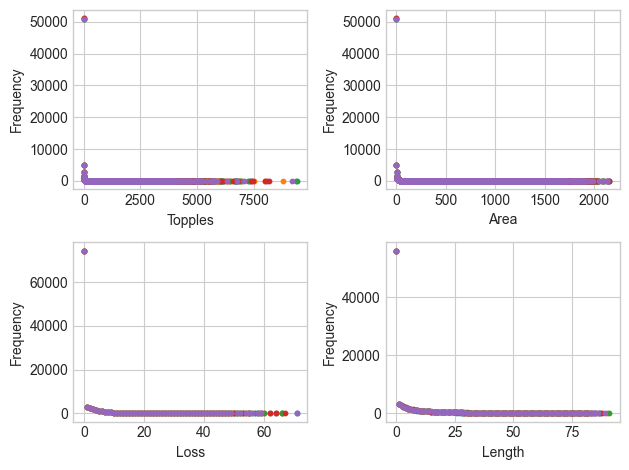
\includegraphics[width=0.6\textwidth]{figures/linear.png}
	\caption{Observed frequencies of Topples, Area, Loss, and Length for five independent simulations on linear axes.}
	\label{fig:linear}
\end{figure}

\section{Spatial Distribution of Sand Heights}

\begin{figure}[htbp]
	\centering
	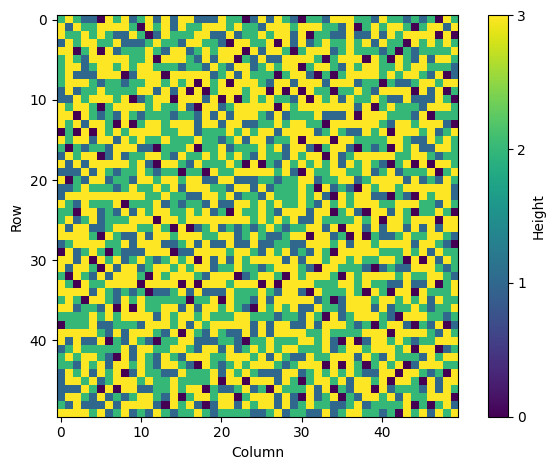
\includegraphics[width=0.4\textwidth]{figures/heat.png}
	\caption{Spatial distribution of sand heights in the final configuration of Pile 5 of the basic model.}
	\label{fig:heat}
\end{figure}

\newpage
\section{Additional Distribution Fits}

\subsection{Power-law Fit For Area}

\begin{figure}[htbp]
	\centering
	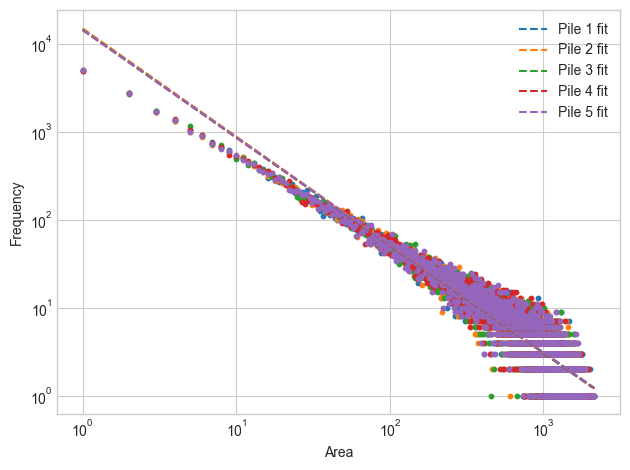
\includegraphics[width=0.8\textwidth]{figures/area_power.png}
	\caption{Observed Area frequencies and fitted power-law curves for five independent simulations on log-log axes.}
	\label{fig:area_power}
\end{figure}


\begin{table}[htbp]
	\centering
	\begin{tabular}{cccc}
		\hline
		Pile & $\alpha$ & MAE & RMSE \\
		\hline
		1 & -1.2198 & 15.7039 & 252.2666 \\
		2 & -1.2276 & 16.9752 & 272.2115 \\
		3 & -1.2251 & 15.8027 & 259.4345 \\
		4 & -1.2215 & 15.6431 & 254.8015 \\
		5 & -1.2206 & 16.1838 & 257.3404 \\
		\hline
	\end{tabular}
	\caption{Power law exponents and fitting errors for the power-law fit to Area.}
	\label{tab:area_power}
\end{table}

\newpage
\subsection{Geometric Fit for Loss Including Zero}
\begin{figure}[htbp]
	\centering
	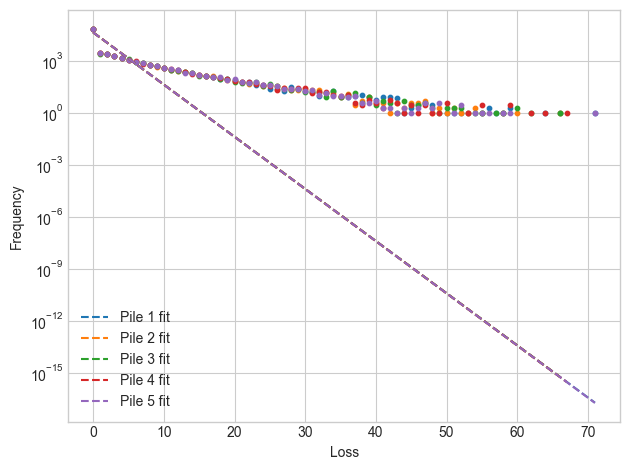
\includegraphics[width=0.9\textwidth]{figures/loss_ge0.png}
	\caption{Observed Loss frequencies and fitted geometric curves including zero for five independent simulations on semi-log axes.}
	\label{fig:loss_ge0}
\end{figure}

\newpage
\subsection{Log-normal Fit for Loss}
\begin{figure}[htbp]
	\centering
	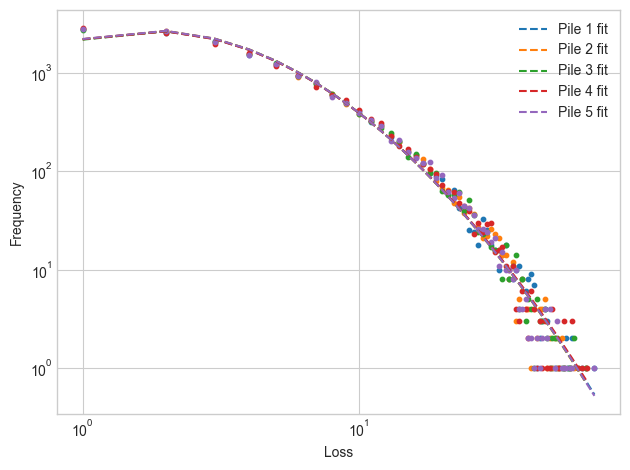
\includegraphics[width=0.9\textwidth]{figures/loss_lognorm.png}
	\caption{Observed positive Loss frequencies and fitted log-normal curves for five independent simulations on log-log axes.}
	\label{fig:loss_lognorm}
\end{figure}


\begin{table}[htbp]
	\centering
	\begin{tabular}{ccccc}
		\hline
		Pile & $\mu$ & $\sigma^2$ & MAE & RMSE \\
		\hline
		1 & 1.3347 & 0.8261 & 26.2768 & 88.9550 \\
		2 & 1.3333 & 0.8187 & 24.9234 & 83.5375 \\
		3 & 1.3377 & 0.8179 & 24.4259 & 83.0422 \\
		4 & 1.3361 & 0.8304 & 30.6826 & 96.2659 \\
		5 & 1.3321 & 0.8215 & 27.6485 & 88.4346 \\
		\hline
	\end{tabular}
	\caption{Estimated log-normal parameters and fitting errors for positive Loss values.}
	\label{tab:loss_lognorm}
\end{table}

\newpage
\section{Additional Correlation Matrices}
\subsection{Correlation Matrix for Pile 2}

\begin{table}[htbp]
	\centering
	\begin{tabular}{lcccc}
		\hline
		& Topples & Area & Loss & Length \\
		\hline
		Topples & 1.000000 & 0.999918 & 0.631324 & 0.962060 \\
		Area    & 0.999918 & 1.000000 & 0.630935 & 0.962363 \\
		Loss    & 0.631324 & 0.630935 & 1.000000 & 0.630655 \\
		Length  & 0.962060 & 0.962363 & 0.630655 & 1.000000 \\
		\hline
	\end{tabular}
	\caption{Spearman correlation matrix for Pile 2.}
	\label{tab:corr_2}
\end{table}

\subsection{Correlation Matrix for Pile 3}
\begin{table}[htbp]
	\centering
	\begin{tabular}{lcccc}
		\hline
		& Topples & Area & Loss & Length \\
		\hline
		Topples & 1.000000 & 0.999921 & 0.627074 & 0.962685 \\
		Area    & 0.999921 & 1.000000 & 0.626732 & 0.962977 \\
		Loss    & 0.627074 & 0.626732 & 1.000000 & 0.625866 \\
		Length  & 0.962685 & 0.962977 & 0.625866 & 1.000000
		 \\
		\hline
	\end{tabular}
	\caption{Spearman correlation matrix for Pile 3.}
	\label{tab:corr_3}
\end{table}

\subsection{Correlation Matrix for Pile 4}
\begin{table}[htbp]
	\centering
	\begin{tabular}{lcccc}
		\hline
		& Topples & Area & Loss & Length \\
		\hline
		Topples & 1.000000 & 0.999919 & 0.627299 & 0.962661 \\
		Area    & 0.999919 & 1.000000 & 0.627074 & 0.962962 \\
		Loss    & 0.627299 & 0.627074 & 1.000000 & 0.626932 \\
		Length  & 0.962661 & 0.962962 & 0.626932 & 1.000000 \\
		\hline
	\end{tabular}
	\caption{Spearman correlation matrix for Pile 4.}
	\label{tab:corr_4}
\end{table}

\subsection{Correlation Matrix for Pile 5}
\begin{table}[!htbp]
	\centering
	\begin{tabular}{lcccc}
		\hline
		& Topples & Area & Loss & Length \\
		\hline
		Topples & 1.000000 & 0.999916 & 0.629966 & 0.961779 \\
		Area    & 0.999916 & 1.000000 & 0.629602 & 0.962091 \\
		Loss    & 0.629966 & 0.629602 & 1.000000 & 0.630056 \\
		Length  & 0.961779 & 0.962091 & 0.630056 & 1.000000 \\
		\hline
	\end{tabular}
	\caption{Spearman correlation matrix for Pile 5.}
	\label{tab:corr_5}
\end{table}

\newpage
\section{Extended Model}

\begin{figure}[htbp]
	\centering
	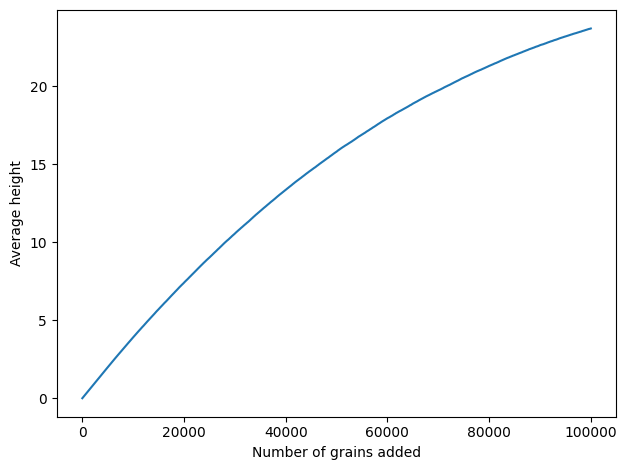
\includegraphics[width=0.6\textwidth]{figures/avg_extend_height.png}
	\caption{Average pile height against the number of grains added.}
	\label{fig:avg_extend_height}
\end{figure}

\begin{figure}[htbp]
	\centering
	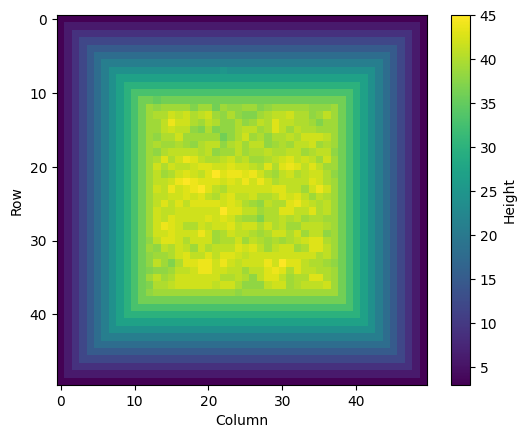
\includegraphics[width=0.6\textwidth]{figures/extend_heat.png}
	\caption{Spatial distribution of sand heights in the extended model.}
	\label{fig:extend_heat}
\end{figure}


